\documentclass[14pt]{extreport}
\usepackage{gost}

\begin{document}

\pagestyle{empty}
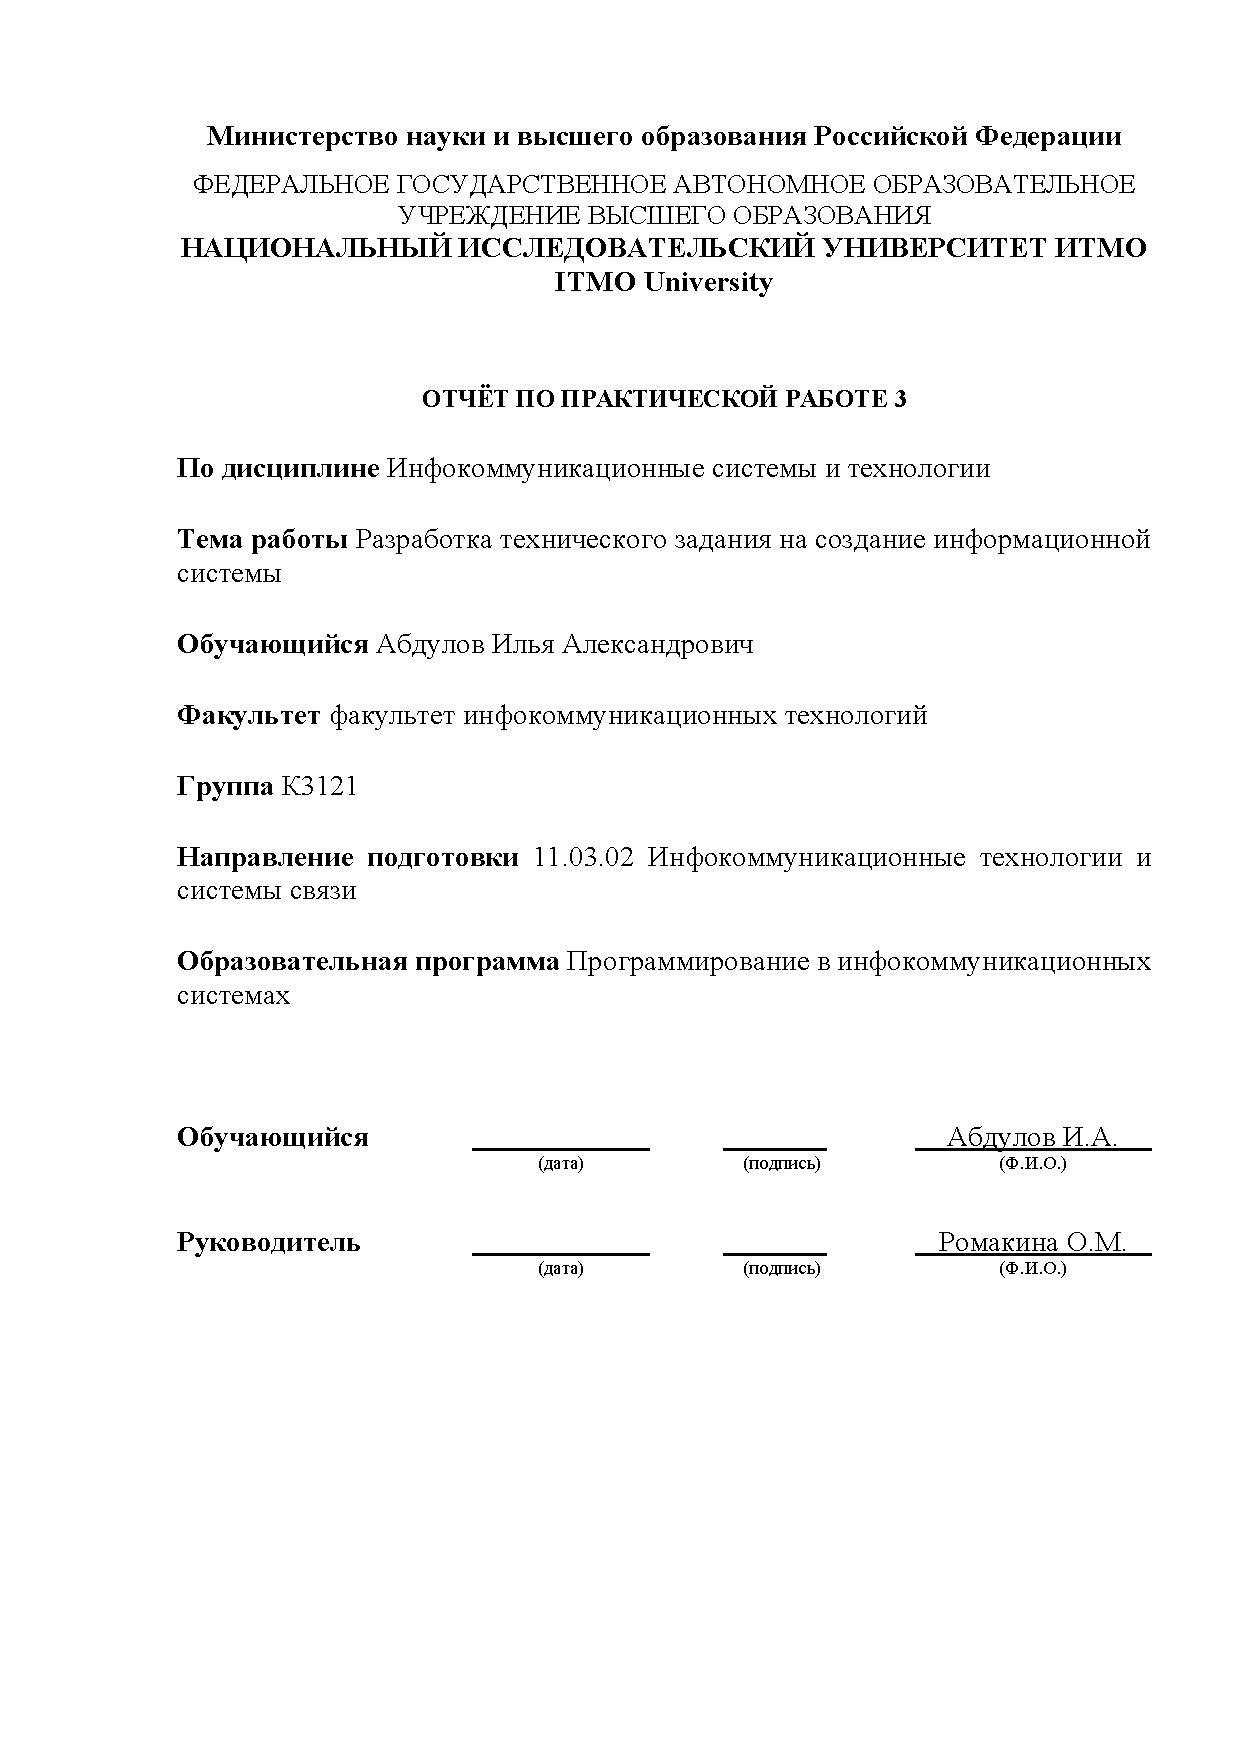
\includepdf{titulCourse.pdf}
\pagestyle{plain}

\tableofcontents

\intro

Практическая работа 3 является актуальной, потому что является описанием основной идеи будущего мобильного приложения. Приложение Better Row представляет из себя приложение, куда пользователь заносит данные своих тренировок, чтобы приложение показывало и сохраняло текущие показатели и прогресс. Использование приложения придаст тренировкам осознанности, что поможет в достижении лучшего результата.

Целью данной работы является описание предметной области функционирования и основной идеи предлагаемой ИС или будущего мобильного приложения. Описание идеи будущей ИС включает: название, назначение, основных пользователей системы, планируемый набор функций для каждого из будущих пользователей, прототип интерфейса будущей системы, обзор аналогов на рынке и обоснование необходимости разработки планируемой системы. В процессе работы будет использован онлайн-инструмент Figma для создания интерфейса приложения.

\chapter{Описание будущей ИС}

\section{Название}

Название приложения {Better Row}\footnote{Лучше Греби – дословный перевод с английского} отражает цель приложения: помочь пользователю улучшить свои показатели и результаты в таком соревновательном виде спорта, как академическая гребля.

\section{Назначение}

Назначение приложения: позволить пользователю сохранять данные о своих тренировках на концепте, чтобы в дальнейшем иметь возможность их просмотреть. Приложение поможет следить за своими показателями тренировок, видеть свой прогресс и иметь возможность поделиться своими результатами с тренером на расстоянии.

\section{Основные пользователи}

Основными пользователями системы будут являться любители академической гребли и участники студенческой гребной лиги России.

\section{Планируемый набор функций}

Для каждого из будущих пользователей планируется реализовать три вкладки в главном меню: результаты и статистика, расписание тренировок, настройки приложения.

Во вкладке результатов пользователь сможет перемещаться по дням и либо просмотреть результаты тренировки в этот день, либо добавить информацию о тренировке. При добавлении тренировки пользователь вводит дистанцию, время, темп заплыва на концепте – обязательные показатели, а также пульс после заплыва – опциональную характеристику для ввода. При просмотре тренировок, которые уже были добавлены к введённым пользователем показателям автоматически добавляется средняя скорость заплыва. Кроме того, реализованы функции просмотра изменения результата по сравнению с прошлыми тренировками.

Во вкладке расписания тренировок будут указанные дни недели, в которые проходят тренировки, время и место занятий секции. Если расписание тренировок поменяется, то, используя функцию, его можно будет изменить.

Во вкладке настроек приложения будут функции смены аккаунта пользователя и сброса данных о всех тренировках.

\section{Прототип интерфейса}

Прототип интерфейса будет реализован в онлайн-инструменте Figma:

\begin{figure}[H]
\centerline{\includegraphics[width=0.43\linewidth]{iphone 8 - 3.pdf}}
\caption{Главная страница}
\label{fig11}
\end{figure}

\begin{figure}[H]
\centerline{\includegraphics[width=0.75\linewidth]{iphone 8 - 1.pdf}}
\caption{Страница результатов и статистики, тренировка 25 октября}
\label{fig12}
\end{figure}

\begin{figure}[H]
\centerline{\includegraphics[width=0.75\linewidth]{iphone 8 - 2.pdf}}
\caption{Страница результатов и статистики, создание тренировки 28 октября}
\label{fig13}
\end{figure}

\begin{figure}[H]
\centerline{\includegraphics[width=0.75\linewidth]{iphone 8 - 4.pdf}}
\caption{Страница расписания}
\label{fig14}
\end{figure}

\section{Аналоги}

Среди аналогов, представленных на рынке приложений можно выделить

\begin{itemize}
\item Watersports Tracker. Приложение, которое предоставляет статистику о тренировке на воде, отслеживая геолокацию смартфона. Приложение бесплатно для скачивания. Пользователи всех водных видов спорта могут воспользоваться данным приложением, чтобы отследить основные показатели такие, как скорость, время, дистанцию, а также маршрут своего заплыва. Плюсы: красивый дизайн, ничего лишнего. Минусы: пользователям требуется приобрести подписку. Вывод: система удобна для пользования на открытом воздухе, но требует покупки подписки.
\item RowingCoach 4.0. Приложение предоставляет статистику и показатели тренировки, отслеживая геолокацию пользователя. Приложение бесплатно для скачивания. Гребцам предоставляется большой список показателей заплыва, с возможностью посмотреть промежуточные результаты на участке пути, отображается маршрут на карте. Плюсы: подробное, с широким функционалом. Минусы: не поддерживается разработчиком. Вывод: приложение предоставляет все данные о тренировке на воде, но уже несколько лет не обновляется разработчиком.
\end{itemize}

\section{Обоснование необходимости ИС}

Все упомянутые в качестве аналогов приложения удобны в использовании, потому что автоматически следят за скоростью и показателями на воде. Но они не дают возможности отслеживать показатели тренировок в спортивном зале. Они берут данные о движении и геолокации смартфона, используя навигацию. Мое приложение необходимо, потому что нацелено на тренировки в закрытом помещении, зале гребли. Все показатели тренировки пользователь заносит в ИС самостоятельно, чтобы увидеть прогресс или упадок показателей своих тренировок.
 
\conclusions

Цель работы была достигнута. Было дано широкое описание будущего мобильного приложения. В отчёте были указаны: название, назначение, основные пользователи системы, планируемый набор функций для будущих пользователей, прототип интерфейса будущей системы, обзор аналогов на рынке и обоснование необходимости разработки системы.

\newpage
\begin{thebibliography}{99}

\bibitem{bib1}Интернет-сервис, который помогает создать прототипы интерфейсов ИС — URL: \url{https://www.figma.com/} (дата обращения 26.10.2022).	
	
\end{thebibliography}

\end{document}
